
\documentclass[journal]{IEEEtran}

%\usepackage[retainorgcmds]{IEEEtrantools}
%\usepackage{bibentry}  
\usepackage{xcolor,soul,framed} %,caption

\colorlet{shadecolor}{yellow}
% \usepackage{color,soul}
\usepackage[pdftex]{graphicx}
\graphicspath{{../pdf/}{../jpeg/}}
\DeclareGraphicsExtensions{.pdf,.jpeg,.png}

\usepackage[cmex10]{amsmath}
%Mathabx do not work on ScribTex => Removed
%\usepackage{mathabx}
\usepackage{array}
\usepackage{mdwmath}
\usepackage{mdwtab}
\usepackage{eqparbox}
\usepackage{url}

\hyphenation{op-tical net-works semi-conduc-tor}

%\bstctlcite{IEEE:BSTcontrol}


%=== TITLE & AUTHORS ====================================================================
\begin{document}
\bstctlcite{IEEEexample:BSTcontrol}
    \title{Project Title}
  \author{Memeber1 Name~\IEEEmembership{Member1 Student ID,}
      Memeber2 Name~\IEEEmembership{Member3 Student ID,}
      Memeber2 Name~\IEEEmembership{Member3 Student ID,}
}  


% The paper headers
\markboth{(NTNU: CSC9005) Data Visualization Final Project (114-1)
}{}


% ====================================================================
\maketitle



% === ABSTRACT ====================================================================
% =================================================================================
\begin{abstract}
Put your abstract here.\\

Length of the proposal and report: 
\begin{itemize}
    \item Proposal 1-3 pages. 
    \item Report: 2-5 pages.
\end{itemize}
\end{abstract}



\IEEEpeerreviewmaketitle



% === Main Content =============================================================
% =================================================================================
\section{Introduction}

\IEEEPARstart{W}{rite} down your introduction section here. Provide a paragraph that introduces the problem your visualization aims to address. Include background information about the issue, a brief description of the target users who care about this problem, and explain why it matters to them or why it is important in their context. Finally, discuss the potential impact or value your visualization could have if it successfully helps these users understand or solve the problem.


\section{Data and Data Processing}

Describe the dataset and the variables that you will visualize. Provide a link to your data source or describe where and how to get the dataset. If you have to preprocess or clean your data before visualize it, briefly describe what you will do and your plan. \\

Note: Consider whether you need to derive new attributes or process the data before creating your visualization. Directly visualizing raw data attributes may not always be effective for certain analytical tasks. 

% \begin{equation}\label{nonideal_rectifier_resistance}
% R(v) =
% \begin{cases}
%     \infty, & v > -V_{tr}\\
%     R_{on}, & v \leq -V_{tr}
% \end{cases}
% \end{equation}

\section{Target User and Task Requirement}

Provide a detailed description of the problem faced by your target users. List (point by point) the specific tasks the tasks users should make it done done to address users' problems, and explain how completing these tasks will help solve or alleviate the users’ challenges.


\section{Visualization Design and Implementation}

Please note that your project should implement a web-based visualization tool using D3.js. If your team has a strong reason for not doing so, you must first discuss it with the instructor and obtain approval.

\subsection{For Proposal}
From your scenario and tasks, design your visualization and interface.
Include and emphasize the visual designs and interaction features you plan to accomplish the tasks.
Your sketch can be hand-drawn (take picture and paste on the report), or mocked up by powerpoint, graphics editor……. Figure \ref{fig:sketch} is an example.
Your sketch could be multiple images to describe your design and plan.
Note: this basic sketch is going to help you to think what you are going to do and your first prototype implementation. It is by no means about what you should submit in the end.

\begin{figure}
  \begin{center}
  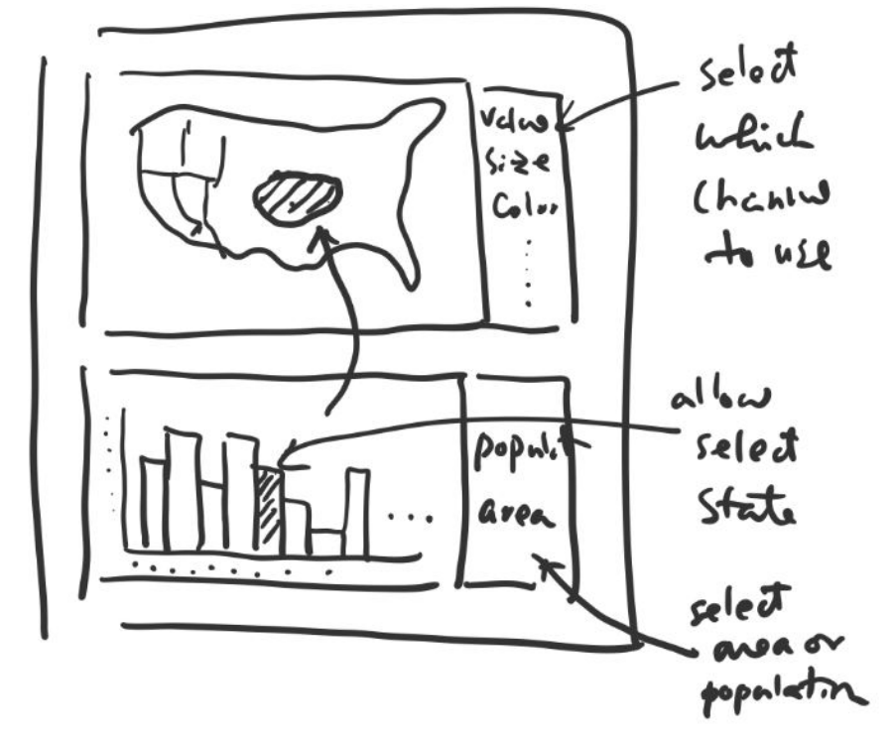
\includegraphics[width=3.5in]{photo/sketch.png}\\
  \caption{Example of one sketch image.}\label{fig:sketch}
  \end{center}
\end{figure}

\subsection{For Final Report}

Please include screenshots and the introduction of your visualization. Provide a detailed explanation of your visualizations and interactions, describing the purpose and design rationale behind each view and interaction.

\section{Use Case}

\subsection{For Proposal}
Give a hypothetical walkthrough of how they accomplish the tasks with your visualization.\\ 

Example: The user examines [plot] and observes [visual patterns], allowing them to obtain [specific information or form a hypothesis]. Consequently, the user performs [an interaction], which updates [specific views]. The user then examines [another plot] and gains [new information, forms a new hypothesis, or confirms a previous hypothesis].\\

Give the explaination why these steps can help users to complte tasks and solve the problem they have.

\subsection{For Final Report}

Similar to what was included in the proposal, but you should provide screenshots of your tool in use to show and explain how users interact with your visualization tool to solve their problem.


\section{Discussion and Conclusion}

This section is not necessary in the proposal.\\

You should discuss the limitations of your work: for example, why your visualization tool might not fully help users complete their tasks effectively, the challenges or difficulties your team encountered in this project, and potential directions for future work to better support users in solving it.


\end{document}


